\documentclass[10pt]{article}
\usepackage[utf8]{inputenc}
\usepackage{cite}

\title{Interfaces Usuário-Máquina: usabilidade e acessibilidade}
\author{Gabriel de Oliveira Pessoa}
\date{Novembro 2019}

\usepackage{natbib}
\usepackage{graphicx}

\begin{document}

\maketitle

\section{Introdução}
As interfaces são aquilo que nos liga direto à maquina, uma forma de interagirmos com ela e darmos comandos. Seguindo esse raciocínio, a cadeira de interfaces usuário-máquina busca formas de facilitar essa comunicação entre o homem e o computador. E a partir de pesquisas se procura a forma mais intuitiva de apresentação de certo produto para seu público, ou seja, como deixar a interface mais intuitiva para seu usuário final, um modo mais claro e direto para que os comando sejam dados.

\begin{figure}[h!]
\centering
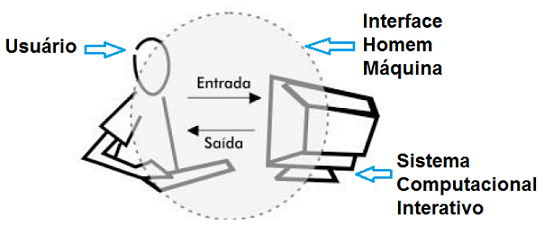
\includegraphics[scale=0.5]{UI.png}
\caption{Representação básica do ciclo usuário-máquina}\cite{hitec}
\label{fig:universe}
\end{figure}

\section{Relevância}
A interface entre o usuário e a máquina é parte fundamental em um software, ela representa a acessibilidade, usabilidade e também o seu design, podendo ser muitas vezes decisivo no sucesso do programa. Por ter tamanha importância no futuro profissional do estudante, a cadeira de interfaces usuário-máquina ensina aos alunos os conceitos básicos de design interativo e também o estimula ter formas criativas de pensamento para solucionar os mais diversos problemas dos diferentes tipos de usuários.  \cite{repositorioufsc} \cite{olharcientifico}

\section{Relação com outras disciplinas}
\begin{itemize}
\item IF679 - Informática e Sociedade: toda a parte de criação de uma nova interface se baseia no seu consumidor final e para isso é necessário entender como atua esse usuário e o que melhor se encaixa no seu uso. \cite{br-ie}
\item IF781 Empreendimentos em Informática - as interfaces atraem o usuário assim como o usuário define a interface, de tal modo que se torna fator decisivo na hora de empreender com um software. \cite{repositorioufsc}
\end{itemize}
\bibliographystyle{plain}
\bibliography{gop2}
\end{document}
